 \subsubsection{UC11 - Visualizzazione delle informazioni utente}
 \begin{figure}[h]
 	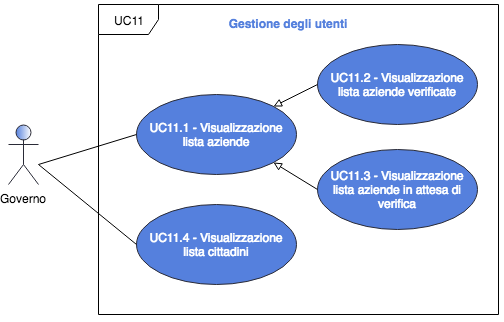
\includegraphics[width=9cm]{res/images/UC11.png}
 	\centering
 	\caption{UC11 - Visualizzazione delle informazioni utente}
 	
 \end{figure}
 \begin{itemize}
 	\item \textbf{Attori Primari}: governo;
 	\item \textbf{Descrizione}: il governo può accedere alle informazioni riguardanti le aziende ed i cittadini che hanno avanzato una richiesta di iscrizione, o che sono già iscritti alla piattaforma. Offre inoltre la possibilità di eseguire delle operazioni su di essi;
 	\item \textbf{Scenario principale}: il governo cerca delle informazioni riguardanti gli utenti della piattaforma e/o esegue delle operazioni su di essi;
 	
 	\item \textbf{Precondizione}: il sistema riconosce che l'utente è autenticato con privilegi governativi e mostra le pagine utili alla ricerca di informazioni;
 	
 	\item \textbf{Postcondizione}: il governo ottiene dal sistema la lista degli utenti dei quali cercava delle informazioni, assieme al set di operazioni che possono essere effettuate su quella tipologia di utente.
 \end{itemize}
 \subsubsection{UC11.1 - Visualizzazione lista aziende}
 \begin{figure}[h]
 	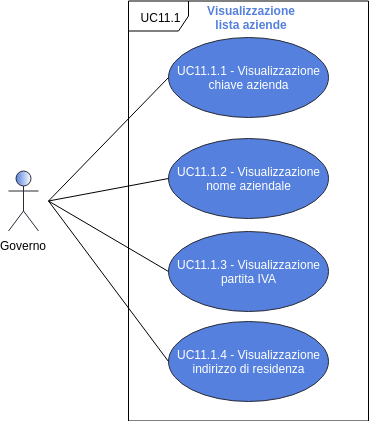
\includegraphics[width=8cm]{res/images/UC11-1.png} 
 	\centering
 	\caption{UC11 - Visualizzazione lista aziende}
 	
 \end{figure}
 \begin{itemize}
 	\item \textbf{Attori Primari}: governo;
 	\item \textbf{Descrizione}: il governo accede ad una lista di aziende, nella quale vengono mostrate tutte le informazioni utili ed operazioni disponibili;
 	\item \textbf{Scenario principale}: il governo può voler ottenere la lista di tutte le aziende iscritte alla piattaforma con le relative informazioni riguardanti l'IVA [UC11.2], oppure può voler controllare, per poi gestire, tutte le aziende che attualmente hanno fatto richiesta di registrazione alla piattaforma [UC11.3]. In generale sono disponibili le seguenti informazioni:
 	\begin{itemize}
 		\item visualizzazione della chiave\glosp Ethereum [UC11.1.1];
 		\item visualizzazione del nome [UC11.1.2];
 		\item visualizzazione della partita IVA [UC11.1.3];
 		\item visualizzazione dell'indirizzo di residenza [UC11.1.4];
 		
 	\end{itemize}
	\item \textbf{Specializzazione}:
	\begin{itemize}
	 	\item \textbf{UC11.2}: il governo vuole ottenere le informazioni relative alle aziende che sono già registrate alla piattaforma. In questo caso saranno presenti anche delle informazioni riguardati la situazione IVA delle aziende;
	 	\item \textbf{UC11.3}: il governo vuole ottenere le informazioni relative alle aziende che sono in attesa di essere verificate, per poter poi usufruire della piattaforma. Da questa vista verranno offerte al governo le operazioni di approvazioni/rigetto della richiesta;
	\end{itemize}
 	\item \textbf{Precondizione}: il sistema riconosce che l'utente è autenticato con privilegi governativi ed ha richiesto le informazioni relative alle aziende;
 	\item \textbf{Postcondizione}: il governo ottiene dal sistema la lista delle aziende cercate con le relative operazioni disponibili.
\end{itemize}
\subsubsection{UC11.1.1 - Visualizzazione chiave azienda}
\begin{itemize}
	\item \textbf{Attori Primari}: governo;
	\item \textbf{Descrizione}: il governo visualizza una lista con tutte le chiavi\glosp Ethereum riguardanti le aziende;
	\item \textbf{Scenario principale}: il governo richiede la lista delle chiavi\glosp relative alle aziende, eventualmente per poi eseguire delle operazioni;
	\item \textbf{Precondizione}: il sistema riconosce che l'utente è autenticato con privilegi governativi ed ha richiesto di ottenere le informazioni sulle aziende;
	\item \textbf{Postcondizione}: il governo ottiene dal sistema la lista contenente tutte le aziende, con associate le relative chiavi\glo.
\end{itemize}
\subsubsection{UC11.1.2 - Visualizzazione nome aziendale}
\begin{itemize}
	\item \textbf{Attori Primari}: governo;
	\item \textbf{Descrizione}: il governo visualizza una lista con tutti i nomi delle aziende interessate nella piattaforma;
	\item \textbf{Scenario principale}: il governo richiede la lista dei nomi relativi alle aziende, eventualmente per poi eseguire delle operazioni;
	\item \textbf{Precondizione}: il sistema riconosce che l'utente è autenticato con privilegi governativi ed ed ha richiesto di ottenere le informazioni sulle aziende;
	\item \textbf{Postcondizione}: il governo ottiene dal sistema la lista contenente tutte le aziende, con associati i rispettivi nomi.
\end{itemize}
\subsubsection{UC11.1.3 - Visualizzazione partita IVA}
\begin{itemize}
	\item \textbf{Attori Primari}: governo;
	\item \textbf{Descrizione}: il governo visualizza una lista con tutte le partite IVA delle aziende interessate nella piattaforma;
	\item \textbf{Scenario principale}: il governo richiede la lista delle partite IVA relative alle aziende, eventualmente per poi eseguire delle operazioni;
	\item \textbf{Precondizione}: il sistema riconosce che l'utente è autenticato con privilegi governativi ed ha richiesto di ottenere le informazioni sulle aziende;
	\item \textbf{Postcondizione}: il governo ottiene dal sistema la lista contenente tutte le aziende, con associate le partite IVA.
\end{itemize}
\subsubsection{UC11.1.4 - Visualizzazione indirizzo di residenza}
\begin{itemize}
	\item \textbf{Attori Primari}: governo;
	\item \textbf{Descrizione}: il governo visualizza una lista con tutti gli indirizzi di residenza delle aziende interessate nella piattaforma;
	\item \textbf{Scenario principale}: il governo richiede la lista degli indirizzi di residenza delle aziende, eventualmente per poi eseguire delle operazioni;
	\item \textbf{Precondizione}: il sistema riconosce che l'utente è autenticato con privilegi governativi ed ha richiesto di ottenere le informazioni sulle aziende;
	\item \textbf{Postcondizione}: il governo ottiene dal sistema la lista contenente tutte le aziende, con associati gli indirizzi di residenza.
\end{itemize}

 \subsubsection{UC11.2 - Visualizzazione lista aziende verificate}
  \begin{figure}[h]
 	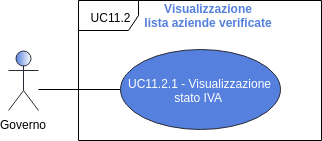
\includegraphics[width=8cm]{res/images/UC11-2.png} %da adattare in larghezza
 	\centering
 	\caption{UC11.2 - Visualizzazione lista aziende verificate}
 	
 \end{figure}
 \begin{itemize}
	\item \textbf{Attori Primari}: governo;
	\item \textbf{Descrizione}: il governo ottiene la lista delle aziende registrate alla piattaforma e già verificate;
	\item \textbf{Scenario principale}: il governo richiede la lista delle aziende registrate e  già verificate;
	\item \textbf{Precondizione}: il sistema riconosce che l'utente è autenticato con privilegi governativi ed ha richiesto di ottenere la lista di tutte aziende già verificate;
	\item \textbf{Postcondizione}: il governo ottiene dal sistema la lista delle aziende registrate e verificate, con associate le operazioni che può effettuare su di esse.
\end{itemize}
\subsubsection{UC11.2.1 - Visualizzazione stato IVA}
\begin{itemize}
	\item \textbf{Attori Primari}: governo;
	\item \textbf{Descrizione}: il governo ottiene la lista dello stato della partita IVA relativo alle aziende registrate alla piattaforma e già verificate. In particolare può osservare se un'azienda è in stato di credito o debito;
	\item \textbf{Scenario principale}: il governo richiede la lista dello stato IVA delle aziende registrate e  già verificate;
	\item \textbf{Precondizione}: il sistema riconosce che l'utente è autenticato con privilegi governativi ed ha richiesto di ottenere la lista di tutte aziende già verificate;
	\item \textbf{Postcondizione}: il governo ottiene dal sistema la lista della situazione IVA delle aziende registrate alla piattaforma. Vengono rese disponibili le operazioni che posso essere attuate su di esse.
\end{itemize}
\subsubsection{UC11.3 - Visualizzazione lista aziende in attesa di verifica}

\begin{itemize}
	\item \textbf{Attori Primari}: governo;
	\item \textbf{Descrizione}: il governo ottiene la lista delle aziende che sono in attesa di essere verificate per poter poi usufruire della piattaforma;
	\item \textbf{Scenario}: il governo richiede la lista delle aziende che sono in attesa di essere verificate;
	\item \textbf{Precondizione}: il sistema riconosce che l'utente è autenticato con privilegi governativi ed ha richiesto di ottenere la lista di tutte le aziende in attesa di verifica;
	\item \textbf{Postcondizione}: il governo ottiene dal sistema la lista delle aziende in attesa di verifica, con associate le operazioni che può effettuare su di esse.
\end{itemize}
\subsubsection{UC11.4 - Visualizzazione lista cittadini in attesa di verifica}
\begin{figure}[h]
	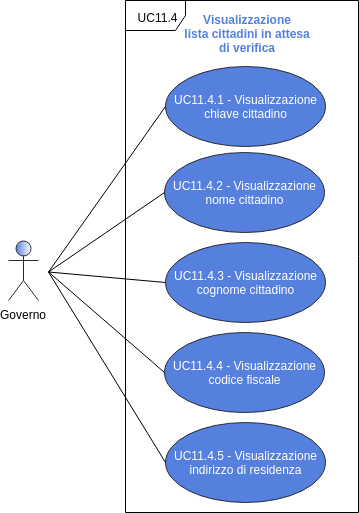
\includegraphics[width=8cm]{res/images/UC11-4.png} %da adattare in larghezza
	\centering
	\caption{UC11.4 - Visualizzazione lista cittadini in attesa di verifica}
\end{figure}
\begin{itemize}
	\item \textbf{Attori Primari}: governo;
	\item \textbf{Descrizione}: il governo ottiene la lista dei cittadini che sono in attesa di essere verificati per poter poi usufruire della piattaforma;
	\item \textbf{Scenario}: il governo richiede la lista dei cittadini che sono in attesa di essere verificati. Le informazioni che vengono rese disponibili sono:
	\begin{itemize}
		\item visualizzazione della chiave\glosp Ethereum [UC11.4.1];
		\item visualizzazione del nome [UC11.4.2];
		\item visualizzazione del cognome [UC11.4.3];
		\item visualizzazione della codice fiscale [UC11.4.4];
		\item visualizzazione dell'indirizzo di residenza [UC11.4.5];
		
	\end{itemize}
	\item \textbf{Precondizione}: il sistema riconosce che l'utente è autenticato con privilegi governativi ed ha richiesto di ottenere la lista di tutti i cittadini in attesa di verifica;
	\item \textbf{Postcondizione}: il governo ottiene dal sistema la lista dei cittadini in attesa di verifica, con associate le operazioni che può effettuare su di essi.
\end{itemize}
\subsubsection{UC11.4.1 - Visualizzazione chiave cittadino}
\begin{itemize}
	\item \textbf{Attori Primari}: governo;
	\item \textbf{Descrizione}: il governo visualizza una lista con tutte le chiavi\glosp Ethereum dei cittadini in attesa di verifica della registrazione;
	\item \textbf{Scenario principale}: il governo richiede la lista dei cittadini in attesa di verifica della registrazione, per poterne visualizzare le chiavi\glosp Ethereum;
	\item \textbf{Precondizione}: il sistema riconosce che l'utente è autenticato con privilegi governativi ed ha richiesto di ottenere la lista di tutti i cittadini in attesa di verifica;
	\item \textbf{Postcondizione}: il governo ottiene dal sistema la lista contenente tutti i cittadini con indicate le chiavi\glosp Ethereum. 
\end{itemize}
\subsubsection{UC11.4.2 - Visualizzazione nome cittadino}
\begin{itemize}
	\item \textbf{Attori Primari}: governo;
	\item \textbf{Descrizione}: il governo visualizza una lista con tutti i nomi dei cittadini in attesa di verifica della registrazione;
	\item \textbf{Scenario principale}: il governo richiede la lista dei cittadini in attesa di verifica della registrazione, per poterne visualizzare il nome;
	\item \textbf{Precondizione}: il sistema riconosce che l'utente è autenticato con privilegi governativi ed ha richiesto di ottenere la lista di tutti i cittadini in attesa di verifica;
	\item \textbf{Postcondizione}: il governo ottiene dal sistema la lista contenente tutti i cittadini con indicati i rispettivi nomi.
\end{itemize}
\subsubsection{UC11.4.3 - Visualizzazione cognome cittadino}
	\begin{itemize}
	\item \textbf{Attori Primari}: governo;
	\item \textbf{Descrizione}: il governo visualizza una lista con tutti i cognomi dei cittadini in attesa di verifica della registrazione;
	\item \textbf{Scenario principale}: il governo richiede la lista dei cittadini in attesa di verifica della registrazione, per poterne visualizzare il cognome;
	\item \textbf{Precondizione}: il sistema riconosce che l'utente è autenticato con privilegi governativi ed ha richiesto di ottenere la lista di tutti i cittadini in attesa di verifica;
	\item \textbf{Postcondizione}: il governo ottiene dal sistema la lista contenente tutti i cittadini con indicati i rispettivi cognomi.
\end{itemize}
\subsubsection{UC11.4.4 - Visualizzazione codice fiscale}
\begin{itemize}
	\item \textbf{Attori Primari}: governo;
	\item \textbf{Descrizione}: il governo visualizza una lista con tutti i codici fiscali dei cittadini in attesa di verifica della registrazione;
	\item \textbf{Scenario principale}: il governo richiede la lista dei cittadini in attesa di verifica della registrazione, per poterne visualizzare il codice fiscale;
	\item \textbf{Precondizione}: il sistema riconosce che l'utente è autenticato con privilegi governativi ed ha richiesto di ottenere la lista di tutti i cittadini in attesa di verifica;
	\item \textbf{Postcondizione}: il governo ottiene dal sistema la lista contenente tutti i cittadini con indicati i rispettivi codici fiscali.
\end{itemize}
\subsubsection{UC11.4.5 - Visualizzazione indirizzo di residenza}
\begin{itemize}
	\item \textbf{Attori Primari}: governo;
	\item \textbf{Descrizione}: il governo visualizza una lista con tutti gli indirizzi di residenza dei cittadini in attesa di verifica della registrazione;
	\item \textbf{Scenario principale}: il governo richiede la lista dei cittadini in attesa di verifica della registrazione, per poterne visualizzare l'indirizzo di residenza;
	\item \textbf{Precondizione}: il sistema riconosce che l'utente è autenticato con privilegi governativi ed ha richiesto di ottenere la lista di tutti i cittadini in attesa di verifica;
	\item \textbf{Postcondizione}: il governo ottiene dal sistema la lista contenente tutti i cittadini con indicati i rispettivi indirizzi di residenza.
\end{itemize}